%!TEX root = ../notes.tex
\section{April 15, 2022}
\subsection{Vector Spaces and Inner Products}
For
\[\bvec{v} = \left( v_1, v_2, \dots, v_n \right)\in\RR^n\]
we can compute $||v|| = \sqrt{v_1^2 + v_2^2 + \cdots + v_n^2} = \sqrt{\bvec{v}\cdot \bvec{v}}$.

For two vectors
\begin{align*}
    \bvec{v} & =\left( v_1, v_2, \dots, v_n \right) \\
    \bvec{w} & =\left( w_1, w_2, \dots, w_n \right)
\end{align*}
both in $\RR^n$, we have
\[\bvec{v}\cdot \bvec{w} = v_1w_1 + v_2w_2 + \cdots + v_nw_n = ||\bvec{v}||\cdot ||\bvec{w}||\cos{\theta}\]
\begin{definition}
    An \ul{orthogonal basis} $\left\{ \bvec{v}_i \right\}$ is a basis with
    \[\bvec{v}_i\cdot \bvec{v}_j = 0 \qquad \text{for $i\neq j$}\]
\end{definition}
\begin{definition}
    An \ul{orthonormal basis} is an orthogonal basis with $||\bvec{v}_i|| = 1$, $\forall i$.
\end{definition}

\begin{figure}[ht!]
    \begin{center}
        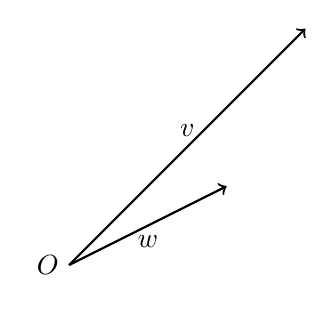
\begin{tikzpicture}
            \draw[->, thick](0,0) node[left]{$O$} -- node[above]{$\bvec{v}$} (3,3);
            \draw[->, thick](0,0) -- node[below]{$\bvec{w}$} (2,1);
        \end{tikzpicture}
    \end{center}
    \caption{Not orthogonal basis. }
\end{figure}

\begin{figure}[ht!]
    \begin{center}
        \begin{tikzpicture}
            \draw[->, thick](0,0) node[left]{$O$} -- node[left]{$\bvec{v}$} (0, 5);
            \draw[->, thick](0,0) -- node[below]{$\bvec{w}$} (3,0);
        \end{tikzpicture}
    \end{center}
    \caption{Orthogonal but not orthonormal }
\end{figure}

\begin{figure}[ht!]
    \begin{center}
        \begin{tikzpicture}
            \draw[->, thick](0,0) node[left]{$O$} -- node[left]{$\bvec{v}$} (0, 4);
            \draw[->, thick](0,0) -- node[below]{$\bvec{w}$} (4, 0);
        \end{tikzpicture}
    \end{center}
    \caption{Orthonormal basis }
\end{figure}

Let $\left\{ \bvec{v}_i \right\}$ be an orthonormal basis, and
\begin{align*}
    \bvec{u} & = a_1\bvec{v}_1 + \cdots a_n\bvec{v}_n \\
    \bvec{w} & = b_1\bvec{v}_1 + \cdots b_n\bvec{v}_n \\
\end{align*}
then
\begin{align*}
    \bvec{u}\cdot \bvec{w} & = \left( \sum_i a_i\bvec{v}_i \right)\cdot \left( \sum_j b_j \bvec{v}_j \right) \\
                           & = \sum_{i, j} a_i b_j \bvec{v}_i\bvec{v}_j                                      \\
                           & = \sum a_i\cdot b_j
\end{align*}

Let $V\subseteq \RR^m$ be a subspace of dimension $n\leq m$ have basis $\{\bvec{v}_1, \bvec{v}_w, \dots, \bvec{v}_n\}$.
\begin{example}
    $V\subseteq\RR^3$, a $2$ dimensional subspace spanned by
    \[(1, 0, -1) \quad (1, -1, 0)\]
    which is the plane $x + y + z = 0$.
    \begin{ques*}
        How do we find an orthogonal basis for $V$?
    \end{ques*}
\end{example}

We use an algorithm called \emph{Gram-Schmidt}.

We first fix $\bvec{v}_1' = \bvec{v}_1$. We then pick a $\bvec{v_2}$ and compute $\bvec{v}_2' = \bvec{v}_2 - \mu_{21} \bvec{v}_1$ where $\mu_{21} \bvec{v}_1$ is the projection of $\bvec{v}_2$ onto $\bvec{v}_1$. What should we select for $\mu_{21}$?

We want $\bvec{v}_1\cdot (\bvec{v}_2 - \mu_{21}\bvec{v}_1) = 0$. This is to say
\begin{align*}
    \bvec{v}_1\cdot \bvec{v}_2 - \mu_{21}(\bvec{v}_1\bvec{v}_1) & = 0                                                          \\
    \mu_{21}                                                    & = \frac{\bvec{v}_1'\bvec{v}_2}{\bvec{v}_1'\cdot \bvec{v}_1'}
\end{align*}
Let's say we get a $\bvec{v}_3$. We have $\bvec{v}_3' = \bvec{v}_3 - \mu_{31}\bvec{v}_1' - \mu_{32}\bvec{v}_2'$.

We now want
\begin{minipage}[t]{.45\textwidth}
    \begin{align*}
        \bvec{v}_1'(\bvec{v}_3 - \mu_{31}\bvec{v}_1' - \mu_{32}\bvec{v}_2')  & = 0                                                                \\
        \bvec{v}_1'\cdot \bvec{v}_3 - \mu_{31}(\bvec{v}_1'\cdot \bvec{v}_1') & = 0                                                                \\
        \mu_{31}                                                             & = \frac{\bvec{v}_1'\cdot \bvec{v}_3}{\bvec{v}_1'\cdot \bvec{v}_1'}
    \end{align*}
\end{minipage}%
\begin{minipage}[t]{.45\textwidth}
    \begin{align*}
        \bvec{v}_2'(\bvec{v}_3 - \mu_{31}\bvec{v}_1' - \mu_{32}\bvec{v}_2')  & = 0                                                                \\
        \bvec{v}_2'\cdot \bvec{v}_3 - \mu_{32}(\bvec{v}_2'\cdot \bvec{v}_2') & = 0                                                                \\
        \mu_{32}                                                             & = \frac{\bvec{v}_2'\cdot \bvec{v}_3}{\bvec{v}_2'\cdot \bvec{v}_2'}
    \end{align*}
\end{minipage}

So in general, we want
\[\bvec{v}_j' = \bvec{v}_j - \sum_{i < j}\frac{\bvec{v}_i'\cdot \bvec{v}_j}{\bvec{v}_i'\cdot \bvec{v}_i'}\cdot \bvec{v}_i'\]

In code, we can implement this as follows (not using \textsf{numpy}):
\lstinputlisting[]{code/linalg.py}

What about with lattices?
*** (pretty diagram)

Any subgroup of a lattice (in particular, of $\ZZ^n$) is itself a lattice.

\begin{definition}
    A subgroup of $\ZZ^n$ is called an \ul{integral lattice}.
\end{definition}
\begin{ques*}
    Is any subgroup of $\RR^n$ a lattice?
\end{ques*}
\emph{Clearly not!} $\RR^n$ itself is not a lattice. $\QQ^n$ is similarly not a lattice.

We want to characterize subgroups of $\RR^n$ that are lattices.
\begin{definition}
    A subset $S\subseteq \RR^n$ is \ul{discrete} if for any $x\in S$: there is some $\epsilon > 0$ such that
    \[\{y\in S\mid ||x - y|| < \epsilon\} = \{x\}\]
\end{definition}
***another pretty picture

\begin{theorem}
    A subgroup of $\RR^n$ is a lattice iff it is discrete.
\end{theorem}
\begin{proof}
    \emph{HW problem.}
\end{proof}